\documentclass[11pt]{scrreprt}

% packages
\usepackage[german]{babel}
\usepackage{eurosym}
\usepackage[utf8]{inputenc}
\usepackage{textcomp}
\usepackage{blindtext}
\usepackage[onehalfspacing]{setspace}
\usepackage{hyperref}
\usepackage{todonotes}
\usepackage{microtype}

% Für vertikale (M) und horizontale (P) Zentrierung des Tabelleninhaltes
\usepackage{array}
\newcolumntype{P}[1]{>{\centering\arraybackslash}p{#1}}
\newcolumntype{M}[1]{>{\centering\arraybackslash}m{#1}}

% include pdf files
\usepackage{pdfpages}

% align text for descriptions
\usepackage{enumitem}
\usepackage{calc}

% move page number down
\usepackage[includefoot,bottom=70pt,margin=1in]{geometry}

% page style
\usepackage{fancyhdr}
\pagestyle{headings}

% serif font in title, chapter and sections
\addtokomafont{disposition}{\rmfamily}

% move titles up to page top
\renewcommand*{\chapterheadstartvskip}{\vspace*{-1cm}}

\begin{document}

\pagenumbering{gobble}
\begin{titlepage}
	\centering
	%\includegraphics[width=0.15\textwidth]{example-image-1x1}\par\vspace{1cm}
	{\scshape\LARGE HTWG Konstanz \par}
	\vspace{1cm}
	{\scshape\Large Business Plan\par}
	\vspace{1.5cm}
	{\huge\bfseries Imagical\par}
	\vspace{2cm}
	{\Large\itshape Vorlesung: Betriebswirtschaftslehre\par}
	\vfill
	erstellt von \\
	\vspace{0.5cm}
	Nico \textsc{Wonneberger} \\
	Sergej \textsc{Birklin} \\
	Pavan \textsc{Singh} \\
	Markus \textsc{Heilig}
	\vfill

    % Bottom of the page
	{\large \today\par}
\end{titlepage}
\tableofcontents
\clearpage

\listoftodos

\pagenumbering{arabic}
\chapter{Executive Summary}



**Finanzierung**: Die monatlichen Kosten werden selbst durch eine pessimistische Einkommensprognose in Deutschland gedeckt. Die anfänglichen einmaligen Kosten werden von den Gründungsmitgliedern eingebracht. Das Fremdkapital vor allem zur Finanzierung weiterer Mitarbeiter und des Marketings soll von Investoren eingebracht werden.
**Geschäftsplanung und Organisation**: Die Funktionsweise der App ermöglicht es unserem Unternehmen, wertvollen Content in hohem Volumen quasi kostenfrei zu erhalten. Alle benötigten technischen Kompetenzen zur Entwicklung der App werden vom Team bereits gestellt. Weitere notwendige Rollen können aufgrund der individuellen Erfahrungen der Teammitglieder ebenfalls gut verteilt werden. Da wir ein digitales Produkt anbieten, können wir standortunabhängig agieren, was weitere finanzielle Vorteile mit sich bringt.
Die Preisgestaltung sieht niedrige Preise für In-App-Käufe vor, welche gemeinsam mit den eigentlichen Alleinstellungsmerkmalen der App weltweit eine breite User-Gemeinde aufbauen sollen. Die User-Gemeinde soll sich ausgehend von Deutschland erst in Europa, dann in den USA und anschliessend auch in östlicheren Regionen verbreiten. Hierfür wird entsprechend dieser Reihenfolge auf gezieltes Online-Marketing und auf Mund-zu-Mund-Propaganda der Foto-Community gesetzt.


Der vorliegende Business-Plan stellt eine Geschäftsidee der Mobile-App \textit{Imagical} vor.
\textit{Imagical} ist eine Fotosharing-App, mit der Benutzer magische Momente in Bildern festhalten und diese der Community zur Verfügung stellen können. 
Die App überzeugt durch mystisches Design und freischaltbare Features.
Die vier Informatikstudenten Pavan Singh, Sergej Birklin, Nico Wonneberger und Markus Heilig realisieren somit die auf dem App-Markt fehlende Lifestyle-Anwendung, welche die beliebten App-Genres ``Foto'' und ``Spiel'' in einer so nie dagewesenen App vereint.

Um genügend Benutzer auf die Plattform zu locken soll die zielgruppengerechte Vermarktung in erster Linie durch soziale Netzwerke, Suchmaschinenwerbung sowie Mund-zu-Mund-Propaganda erfolgen. 
	
\chapter{Produkt und Dienstleistung}

Bei unserem Produkt handelt es sich um eine Fotosharing App. Damit ähnelt sie bekannten Apps wie Instagram und anderen großen Apps. Ein Markt für diese Art Apps ist existiert also. Einige wichtige Unterschiede gibt es, die unsere App von den existierenden Apps unterscheidet.
Um in die App zu kommen muss man einmal pro Tag ein Foto machen und hochladen. Öffnet man die App und hat an diesem Tag noch kein Foto hochgeladen, muss man erst eines machen und hochladen, bevor man die Bilder der Anderen sehen, oder sonst irgendwas machen kann. Das führt dazu, dass die App davor geschützt ist, aus mangel an Content uninteressant zu sein. Zum einen, weil ein neuer Benutzer zuerst etwas zur App beiträgt, bevor er überhaupt sieht, wie belebt die App ist. Zum anderen wird so auch mit wenigen Benutzern um einiges mehr Content generiert als bei anderen Sharing-Apps.
Man kann keine Fotos aus der Galerie hochladen, nur welche, die man mit der App aufnimmt. Dadurch wird verhindert, dass Benutzer das selbe Bild öffters zu sehen bekommen kann und dadurch gelangweilt werden könnte. Außerdem wirken die Bilder in der App dadurch authentisch und exklusiv. Bilder die in unserer App zu sehen sind, können nicht in anderen Apps gefunden werden.
In der App kann man die Bilder aller anderen User durchstöbern und ansehen. Der hauptsächliche Kundennutzen der App gegenüber den Konkurenten, ist die Art an Bildern, die gezeigt werden. Man folgt nicht berühmten Persöhnlichkeiten oder bekommt Bilder, die im Internet gefunden wurden. Statt dessen sieht man nur die beliebtesten Bilder, die Menschen mit der App selbst gemacht haben. Da jeder der die App benutzt auch selbst Bilder hochläd, entsteht automatisch ein Gefühl der Zugehörigkeit. Das trägt unheimlich der Kundenbindung zu, was für das Geschäftsmodell sehr wichtig ist.
Schaut man mit der App ein Bild in der Detailansicht an, muss man dieses Bewerten, um zurück zur Bilderübersicht zu kommen. Dadurch werden Alle Bilder von vielen Bewertet und schlechte und gute Bilder können einfach unterschieden werden. Zudem kann die Auswahl der Bilder, die jedem Bentzer angezeigt werden, personalisiert werden. Bei vielen Bentzern ist die Anzahl der neuen Bilder pro Tag hoch. Durch die Personalisierung können sich dann unterschiedliche Communities inerhalb der App bilden, die jeweils eine etwas andere Art von Bildern bevorzugen.
Das Bewerten aller Bilder ist zudem wichtig, weil ein Benutzer Punkte für seine Bilder bekommt, je nach dem wie gut diese bewertet werden. Alle normalen Features, die über die oben genannten Grundfeatures hinaus gehen, (z.B. Kommentare schreiben, Filter für Fotos benutzen, username angeben, ...) müssen erst für Punkte freigeschaltet werden. Dadurch haben die Benutzer den Ansporn nur gute Bilder zu machen.
Das freischalten von dingen mittels Punkten in einer App kennen Benutzer eher von Spielen. Bei einer anderen App könnte man zuerst meinen, dass es ein Nachteil wäre, dass man als Benutzer am Anfang nicht alles machen kann, was andere können. Jedoch ist das Prinzip des Fortschritts sehr Spaßig. Die Benutzer haben einen Ansporn sich aktiv mit der App zu beschäftigen.
Die App wird kostenlos angeboten. Das Geschäftsmodell der App basiert auf In-App käufen. Die Punkte die zur Freischaltung von Features benötigt werden können in der App gekauft werden. Wegen des starken Gefühls der Gemeinschaft in der App und der involvierung jedes Benutzers, ist es den den meisten wichtig, alle Möglichkeiten der App nutzen zu können. Aus diesem Grund wird ihnen ein In-App kauf ihr Geld wert sein.
Die App ist am Ende der Konzeptionsphase und muss nun nur noch umgesetzt werden. Wegen der Natur der freischaltbaren Features kann jedech auch nach dem Release der App immer weitere Funktionalität hinzugefügt werden. Damit wird dann gleichzeitig der Drang nach genug Punkten erhöht, um diese benutzen zu können.
\chapter{Markt und Wettbewerb}
Laut einer aktuellen Analyse von \textit{Statista} benutzen in Deutschland ca. 50~Millionen Menschen ein Smartphone. Weltweit sind es sogar über 3.5~Milliarden Menschen und rein theoretisch entspricht das der Anzahl möglicher Kunden. Natürlich ist das reale Marktpotenzial deutlich geringer, da zum einen Smartphonebenutzer unterschiedliche Interessen haben und sich möglicherweise Applikationen wie \textit{iMagical} nicht herunterladen. Auf der anderen Seite gibt es Anbieter, die bereits in diesem Markt aufgestellt sind und konkurrieren. Um sich einen besseren Überblick des Marktpotenzials zu verschaffen, soll dieses Kapitel das Marktsegment, sowie dessen Konkurrenten genauer analysieren.

Die Geschäftsidee fokusiert sich nicht auf eine bestimmte Altersgruppe, da heutzutage über Altersgrenzen hinweg Menschen gerne Fotos machen und diese teilen. Nichtsdestotrotz liegt aber das Augenmerk auf Benutzer zwischen 15 und 35 Jahren. Diese Benutzer bilden die wichtigste Zielendgruppe und erlauben eine genauere Marktsegmentierung. Dazu gehört z.B., dass sowohl weibliche, als auch männliche Kunden angesprochen werden sollen. Ferner soll die Applikation nicht nur in Europa und Amerika vermarktet werden, sondern auch in Asien. Ein Grund hierfür ist eine maximale Interessensgruppe aufzubauen, da das Teilen von privaten Momenten auch in dieser Benutzergruppe nicht durchwegs Zustimmung findet.

Um das Marktpotenzial herzuleiten muss zunächst die Größe der Zielendgruppe bestimmt werden. Eine weitere Studie von \textit{Statista} besagt, dass diese Gruppe einem Anteil von ca. 45~\% entspricht, sodass aktuell 1.58~Milliarden potenzielle Benutzer in Frage kommen. Als logische Annahme solll gesagt werden, dass ein Benutzer täglich durchschnittlich 1~Cent an Einnahmen wie z.B. durch In-App Käufe oder Werbung einbringt. Durch diese Berechnung gelangt man auf ein jährliches Gesamtpotenzial von 5.75 Milliarden~€.

Nachdem nun das potenzielle Marktvolumen beziffert wurde, soll auch ein Blick auf die aktuellen Wettbewerber geworfen werden. Für die Darstellung der Wettbewerber soll die vereinfachte Stärken-Schwächen Analyse (Tab. 3.1) herangezogen werden.

Die vereinfachte Stärken-Schwächen Analyse zeigt, dass der Markt noch Potenzial bietet, sofern man natürlich die Schwächen der Konkurrenz ausnutzt und diese in seine eigenen Stärken umwandelt.

\begin{center}
	\begin{table}[htbp!]
	\centering
		\begin{tabular}{| M{2cm} | M{5cm} | M{5cm} | M{3cm} |}
		\hline
			\textbf{ } & \textbf{Stärken} & \textbf{Schwächen} & \textbf{Selbstvergleich} \\ \hline
			Instagram 
			& \begin{itemize}
				\item[]
				\item viele Benutzer
				\item Verbindung anderer sozialer Netzwerke
			\end{itemize}
			& \begin{itemize}
				\item nur für iOS \& Android
				\item Konkurrenten senken direkt Marktanteil
				\item viele qualitativ schlechte Bilder
			\end{itemize} 
			& -+
			\\ \hline
			
			Twitter 
			& \begin{itemize}
				\item viele Benutzer
				\item im Business Bereich beliebt
				\item sehr lebendig
			\end{itemize}
			& \begin{itemize}
				\item beschränkte Zeichen pro Nachricht
				\item kein solides Ertragsmodel
			\end{itemize} 
			& +
			\\ \hline
			
			Pinterest 
			& \begin{itemize}
				\item einfache Navigation
				\item qualtitativ hochwertige Bilder
			\end{itemize}
			& \begin{itemize}
				\item viel Spam
				\item Technik nicht ausgereift
			\end{itemize} 
			& ++
			\\ \hline
		\end{tabular}
		\caption{Vereinfachte Stärken-Schwächen-Analyse}
		\label{table:simpleSwot}
	\end{table}
\end{center}
\chapter{Marketing und Vertrieb}

Das Ziel unseres Marketings soll sein, durch die Anstrengungen des Chief Marketing Officers bis in einem Jahr 10.000 aktive User zu generieren.
Die App hat auf den ersten Blick nur Nachteile für den User. Der User muss Bilder machen um die App zu benutzen und muss Features erst freischalten, die er in anderen Fotosharing Apps standardmäßig hat. Genau das soll aber durch das Marketing als besonderheit positiv aufgezeigt werden.
Die App ist zwar kostenlos aber wegen der In-App käufe in gewisser Weiße teurer als die konkurierenden Apps. Auch die Features der App sind wie bereits erwähnt nicht unbedingt besser als die der Konkurenten. Aus diesen Gründen werden wir mit der App eine Nischenstrategie fahren.


\section{Marketing-Ziel}

Das Ziel unseres Marketings ist es, innerhalb eines Jahres 10.000 aktive User weltweit zu generieren.

\section{Marketing-Strategie}

Auf den ersten Blick könnte sich fälschlicherweise der Eindruck ergeben, als hätte die Funktionsweise der App Nachteile für den Nutzer. Der User muss Bilder machen, um die App zu benutzen. Ausserdem muss er Features erst freischalten, die er in anderen Fotosharing Apps standardmäßig hat. Genau diese Aspekte sollen aber durch das Marketing als Vorteile gepriesen werden.
Die App kann zwar kostenlos runtergeladen werden, ist aber wegen der In-App-Käufe genau genommen teurer als die konkurierenden Apps. Die App hat zwar besondere Alleinstellungsmerkmale, diese sind aber auf dem ersten Blick nicht einfach zu erkennen. Aus diesen Gründen werden wir mit der App eine Nischenstrategie fahren und beim Marketing einen besonderen Augenmerk darauf legen, dass diese Alleinstellungsmerkmale klar vermittelt werden.

\section{Markteinstiegsbarrieren}

Die größte Markteintrittsbarriere ist die Produktdifferenzierung. Die meisten Smartphone-User, die gerne ihre Fotos teilen, machen das bereits über andere Apps. Jedoch benutzen solche Smartphone-User gerne mehrere Fotosharing-Apps gleichzeitig, um mit den Fotos noch mehr Menschen zu erreichen. Dieser Punkt kann beim Markteintritt helfen, da sie mit unserer Fotosharing-App vor allem im Nischensegment noch mehr Leute erreichen können. Der Aspekt des Nischensegments bringt noch einen weiteren wichtigen Vorteil mit sich: User, die bewusst nur Fotos aus dem Nischenbereich suchen, finden mit unserer App erstmalig eine solche Gelegenheit. Anders formuliert könnte unsere bessere App aufgrund dieses Nischen-Alleinstelllungsmerkmals besser passen als die Apps der Konkurrenz, was sie noch stärker dazu führen könnte, auf unsere App umzusteigen bzw. diese mitzubenutzen.


\section{Kundenbindung}

Unsere App möchte in erster Linie nicht nur User gewinnen, sondern diese auch langfristig an sich binden. Das ist darauf zurückzuführen, dass tendentiell eher die langfristigen User dazu neigen, In-App-Käufe zu tätigen. Aus diesem Grund ist die Kundenbindung sehr wichtig für unser Produkt. Um diese langfristige Bindung zu ermöglichen, soll im Marketing kommuniziert werden, dass es sich um eine Lifestyle-App handelt. Dadurch werden Benutzer angeworben, die an einer längeren Benutzung der App interessiert sind.
Des Weiteren soll den Benutzern unserer App und potentiellen neuen Usern gezeigt werden, dass die Macher der App sich um die Benutzer kümmern. Deshalb soll auf Bewertungen und Kommentaren im App-Store und auf dem Google Play Store immer geantwortet werden und auf Verbesserungsvorschläge eingegangen werden.

\section{Marke}

Die Marke der App zielt auf junge Leute ab, die sich der Natur oder dem Mysteriösen hingezogen fühlen. Im Anhang befindet sich der Creative Brief der App, der diese Marke beschreibt.
Der Name \textit{Imagical} geht aus dieser Marke hervor. Er setzt sich aus den Englischen Wörtern "image" und "magical" zusammen. Englisch ist der Name, um die App international vermarkten zu können.
Mit dieser Marke ist es einfach zu kommunizieren, wieso die User gezwungen sind ein Bild hochzuladen. Die Idee ist hierbei, dass die User jeden Tag einen magischen Moment finden und festhalten sollen. Die App wirkt damit so, als würde sie die User nur dazu motivieren wollen auf magische Momente zu achten.
In der App wird die Marke mit der Metapher eines Himmels realisiert. Die Bilder die durchsucht werden können räpresentieren Wolken am Himmel. Das funktioniert, da die Bilder in der Übersicht verschwommen dargestellt werden. Die Punkte, die man in der App sammelt, sowie die Features die man mit diesen Punkten freischalten kann werden ebenfalls als Teile des Himmels dargestellt. Sie sollen in die Marke der App passen und auf keinen Fall so wirken, als seien sie ein aufgesetzes System um Geld zu verdienen. Deshalb müssen die freischaltbaren Features mit Kryptischen Namen benannt werden und abstrakte Icons besitzen. Dadurch wirken sie konsistent mit der App in ihrer geheimnisvollen Art.
Im der Werbung wird auf die freischaltbaren Features und die In-App käufe kein Focus gelegt, da sie von Außen eher als Nachteil gesehen werden. Bei genügend langer Benutzung wird der Vorteil der freischaltbaren Features jedem User klar.

\section{Werbemaßnahmen}

Als Werbemaßnahmen werden wir zum einen gesponsorte Beiträge auf Facebook, sowie Google Adwords Werbung. In beiden Fällen können die Zielgruppen genau bestimmt werden. Das ist sehr hilfreich, da unser Produkt nur bestimmte Menschen anspricht. Und weil wir ein digitales Produkt haben, macht es auch Sinn, dass die Werbung auch an diejenigen geht, die sich in der Digitalen Welt bewegen.
Bei Google Adwords wird pro Klick gezahlt. Es muss deshalb darauf geachtet werden, dass unsere Werbebanner nicht besonders viele Klicks bekommen, sondern, dass jeder der dem Link folgt auch genau weiß, was beworben wird und ob es auf ihn passt. Ein Maximalwert für die Kosten kann angegeben werden. Diesen sollten wir bei etwa 10€ am Tag festlegen und über 50 Tage laufen lassen. So können wir versuchen beständig neue Benutzer anzuwerben. Dadurch wird der Content der App auch beständig gefüllt, denn jeder neue Benutzer trägt als erstes etwas dazu bei. So kann verhindert werden, dass Benutzer die App wegen Mangels an neuen Bilder nach einer Weile uniteressant finden.
Das selbe gilt für die Facebook Beiträge. Hier kann der Preis der Werbung in ähnlicher Form angegeben werden. 10€ pro Tag über 50 Tage sollten auch hier investiert werden.

\section{Mundpropaganda}

Diese Werbemaßnahmen sind nicht dafür gemacht, alle möglichen User zu erreichen. Die Marke der App und das Gemeinschaftsgefühl das bei den Benutzern hervorgerufen wird ist in einer Bannerwerbung schwer in seiner Ganzheit einzufangen. Dazu eignet sich Mundpropaganda um einiges Besser. Die Werbung ist deshalb dazu ausgelegt eine genügend hohe Anzahl an Nutzern zu gewinnen, um den Content der App interessant zu machen. Die eigentliche Verbreitung geschieht dann von der weiterempfehlung der begeisterten Benutzer.
Die bieden Werbekampangen sollten dabei gleichzeitig und nach release der App starten. Die App muss bereits im App-Store sein, damit diejenigen die auf die Werbung aufmerksam werden die App auch sofort herunterladen können. Die App muss dann bereits mit Content gefüllt sein, der in der Betaphase der App entstanden ist. Laufen die beiden Kampangen gleichzeitig und über einen längeren Zeitraum ist die Chance hoch, dass manche Potenziellen Kunden die Werbung mehrmals auf unterschiedlichen Wegen zu sehen bekommt. Das führt dazu, dass diejenigen der Marke ein höheres Vertrauen schenken und eher dazu geneigt sind unser Produkt auszuprobieren.

\chapter{Geschäftsmodell und Organisation}


Geschäftsmodell und Organisation

sehr kurze Beschreibung Geschäftsmodell:
Die (weltweiten) User können sich die Fotoapp kostenlos herunterladen und sind angehalten pro Login-Session mindestens ein
besonderes Foto (kostenfrei) hochzuladen. Somit werden die besonderen Fotoinhalte, welche letzten Endes weitere User anlocken sollen, von der App-Community kostenlos frei gesteuert,
ohne das wir für diese wertvollen Inhalte bezahlen. Je mehr likes einzelne Fotos erhalten, umso mehr Punkte erhält der Hochlader.
Diese Punkte kann er für sonst zahlungspflichtige Features eintauschen oder auch als Eigenmarketing seinen Kanal benutzen. Andere User können besondere Inhalte/Features gegen Punkte/Geld freikaufen,
wodurch das Unternehmen sein Geld verdient.

Kernaktivität: Bereitstellung einer Sharing-Plattform auf der ganz besondere Foto-Inhalte von privaten Usern veröffentlicht werden können.


Das Produkt (Fotoapp) wird hochskaliert und weltweit angeboten. Die interessanten Fotoinhalte werden von den User mindestens bei jedem
Login in die App erstellt, auch weitere Fotos können geladen werden -> skaliert sehr hoch. 
•Ressourcen: Beschreiben Sie, welche Ressourcen notwendig sind, damit Ihr Geschäftsmodell funktioniert. 
Diese Ressourcen können folgender Art sein: physisch (z. B. Gebäude, Maschinen, Fahrzeuge), geistiges Eigentum
 (z. B. Patente, Marken, Software, Kundenprofile) oder finanziell (z. B. Cash, Kreditlinie, Investment) sowie 
 Kompetenzen und „Know-how“ beispielsweise vom Gründerteam und/oder Personal mit spezifischen Qualifikationen.
 
 xxxxxxxxx
 notwendige Ressourcen:
 -physisch:(z. B. Gebäude, Maschinen, Fahrzeuge)
 - geistiges eigentum:z. B. Patente, Marken, Software, Kundenprofile)
  nicht patentierbar, keine besonderen algorithmen, ausgang eu, nicht usa
 -finanziell (z. B. Cash, Kreditlinie, Investment)
 -Kompetenzen und „Know-how“ beispielsweise vom Gründerteam und/oder Personal mit spezifischen Qualifikationen:
 Ressourcen: 
 vorerst stellen die vier Mitglieder des Teams alle benötigten technischen Ressourcen, da alle Informatiker sind:
 -wichtige Fachbereiche: Entwicklung (Backend/Frontend), Deployment, Performance, Testing, Dokumentation:
 
 Entwicklung verteilt sich über alle:
 Markus:Backend,Performance
 Sergej:Backend,Deployment
 Pavan:Frontend,Testautomatisierung
 Nico:Frontend,Dokumentation
 1-2 Designer: Frontend/Gui
 
 Vorkenntnisse Erfahrungen: Alle AIN-Studenten, viel erfahrung aus Projekten
 Markus:Entwickler bei EADS (backend-erfahrung), Informatik Ausbildung
 Sergej:Backend,Deployment (backend und app entwickler-erfahrung), Marketing
 Pavan:Frontend,Testautomatisierung (testautomatisierung und fe erfahrung,startup-erfahrung (pitching,gründung, finanzen, rechtliches, organisation)), Finanzen
 Nico:Frontend,Dokumentation (mediendesign erfahrung)
 1-2 Designer: Frontend/Gui
 
 Organisation: Scrum, rollenverteilung grob (flache hierarchien)
 entsprechende Rollen vorerst nach aussen (zwangs eines zunächst kleinen Teams):
 technischer vorstand nach aussen (CTO):Markus
 geschäftsführend nach aussen: Pavan 
 
 entsprechend parallel zusätzliche rollen:
 Markus:erschliessung zukünftiger technologischer entwicklungen
 Sergej: Marketing und Vertrieb
 Pavan:finanzen, geldbeschaffung, rechtliches
 Nico:Kundenbetreuung
 
 extern:
 -sobald investorengelder da:
 -auslagerung marketing und vertrieb an externe virma
 -auslagerung kundenbetreuung
 -rechtliche fragen für landesspezifische Gesetzgebung (Datenschutz und sonstiges)
 - zusätzliches mentoring durch eigene investoren
 - lokale vertriebsmanager nach etablierung
 
 
 Die Kompetenzen erstrecken sich über die eingesetzte Programmiersprache und Frameworks, Deployment durch Studium und praktische Erfahrung (PSS),
 die Testkompetenzen ebenfalls, Dokumentation der Software und Entwicklungsorganisation (Scrum)
 Zusätzlich ist im Team Teammitglieder Startup-Erfahrung und Pitch-Erfahrung, vorhanden, sodass man über die ein oder anderen Stolpersteine bereits bekannt sind, genauso
 wie die Wichtigkeit des Mentorings, für das die Investoren natürlich gezielt ausgesucht werden sollen (nicht nur finanzielle Hilfe, sondern auch Domänen-Kompetenz und Hilfe bei Markteintrittsbarrieren
 und professionelle Unternehmensentwicklung und Führung)
 Was fehlt, wäre das Geld für Marketing,es soll versucht werden, dieses einzuholen
 -bargeldbestände können aktuell beschränkt werden auf knapp 500-1000€ für Reise und Unterkunft zu Investoren/Messen (initialkosten für investorenanwerbung)
 -weiterbildungskosten (derzeit abgedeckt), spätere weiterbildung nicht auszuschliessen (wirtschaftlich/technisch)
 -materialkosten für werbematerial auf messen oder für investoren
 
 zusatz:
 Unternehmerteam, Management und Personal
-möglcihst kleine Teamgrösse: aktuell vier personen, (ohne designer)
-leute kennen sich schon lange, verstehen sich gut, haben schon gemeinsam projekte betreut
-alle vier sind überzeugt von der idee und möchten diese gemeinsam vorantreiben.
-alle vier arbeiten unabhängig, können hürden bewältigen.
-so überzeugt, dass jeder 2000 € mit einbringt.
 
 Partnerschaften:
 Partnerschaften wird es zuerst mit Investoren zwangsläufig geben.
 Erwartungen an diese: Startup Kompetenz im Medienbereich/Werbebereich.
 Kompetenzen in Markteinführung, Weiterenticklung, marketing und Vertrieb.
 
 technische Partnerschaft: Server von Amazon. 
 Eigenschaften: gute flexible Kostenstruktur, zuverlässige in Europa platzierte 
 Server für besseren Datenschutz.Hierfü werden natürlich Kosten fällig.
 
 Partnerschaften können sich evtl aus den Vertriebswegen ergeben, dass Firmen
 gegen kleinen Anteil zu festgelegten Konditionen /festgelegte Art unser Unternehmen vermarkten
 bzw. aktiv nutzen und somit ihre eigene Community auf unsere App aufmerksam machen.
 
 Möglicherweise Partnerschaften mit besonderen Erlebnisunternehmen (Otto-200E Erlebnisgutscheine), Reiseuntrnehmen,
 mit denen ergeben sich synergien. Das ganze ist allerdings nur ein Ausblick.
 Es wird nicht nur werbung für unsere app gemacht, die ja besondere momente festhält, sondern auch für die unternehmen selbst,
 da diese besondere momente bewerben.
 
 z.b. mit ausrüsterfilmen: wie z.b. canon spiegelreflexkameras oder samsung-hersteller mit ganz besonders guter kamera, die geeignet istu
 um besondere momente festzuhalten auf unserer app
 solche Unternehmen haben ganz andere kernaktivitäten, die sich mit unseren perfekt ergenzen.
 somit keine konkurrierende Interessenverfolgung, denn diese unternehmen konkurrieren z.b.
 auch nicht mit unseren konkurrenten (Instagram, pinterest, etc.)
 
 -make or buy:
 für die kernaktivitäten bestehen derzeit alle benötigten technischen kompetenzen im eigenen team.
 -für das marketing könnte eine marketing-firma engagiert werden, bzw. vertriebsleute eingestellt werden,
 da professioneller marketing/vertrieb nicht zu unseren kernkompetenzen gehört.
 -später supportdienst outsourcen

 kostenstruktur: wichtigste kostentreiber:
 marketing/vertrieb
 die meisten leute haben gute smartphones mit top-ausgestatteten kameras, daher ist das keine sorge
 
 -value proposition/nutzenversprechen: wir ermöglichen das sehen und teilen von ganz besonderen momenten im fotoformat.
 
 •Kundensegmente: Beschreiben Sie, wen genau Sie als Kunden erreichen und bedienen wollen.
 -kundensegment: erstlinig die junge generation: ab 16 bis 35, aber natürlich auszuweiten für alle alterklassen, wobei
 die älteren natürlich nicht so häufig auf smartphones/social networks herumtreiben. 
 
 aus diesem grund wird auch gezielte werbung für diese Zielgruppe gemacht, siehe marketing.
 Die Kunden erstrecken sich über den Globus, allerdings macht es sinn sich auf die Kundschaft entsprechend unserer Marketingstrategie zu konzentrieren,
 sprich:geographischer Aspekt der Kunden: Deutschland, UK, Frankreich, Spanien, wenig gelder in andere europische länder,
 hauptgelder schon eher dann in usa, da in europa über die grossen länder bereits mund zu mund propaganda betrieben wird 
 und man hier an werbegeldern etwas sparen kann für die restlichen verbleibenden länder
 
 -Vertriebs/Kommunikationskanäle:
 Über facebook zielgruppe wählen, dann bezahlen, rest übernimmt facebook.
 Kriterien für facebook-wahle zum einstellen:
 Alter: 16-34
 -hobbys/interessen: reisen, #life, #happiness, #travel, #adventure, landesspezifische hashtags #love,#paris,#berlin,etc.
 -hauptsächlich europa, Nordamerika asien  zuerst in dieser reihenfolge.
 damit sollte schon genug marketing geld fürs erste ausgebucht sein.
 je etablierter die app wird (schneeballeffekt), umso besser läuft die mund zu mund propaganda
 umso mehr wird der vertrieb von selbst statt finden. dennoch: wenn der cashflow stärker wird (gewinne nicht unbedingt)
 kann man das geld gleich für weitere werbungen einsetzen, vor allem verstärkt in asien und in den anderen noch nicht erfassten 
 kontinenten/ländern, bevor hier nachahmer aktiv werden. Geschwindigkeit zählt am anfang mehr, dadurch sind langfristige rentabilitäten eher garantiert (schutz vor nachahmer)
 
 
 -spätere vertriebswege über synergetische Partnerschaften:
 (optimalzustand): Iphone-Werbung oder gutschein werbung, die in ihren Werbungen unsere app einblenden
 bzw. die app erwähnen: schöne momente festhalten und teilen (hier wird unsere app kurz eingeblendet)

 -spätere vertriebswege über hotels (hotelketten): hochzeiten bei hilton als besondere momente festhalten.
 werbung für hotelkette, für uns gratis-werbung. Um auf solche unternehmen verstärkt einzugehen und nicht nur weltketten
 sondern auch lokal fest verwurzelte international bekannte niederlassungen/events zu erreichen (oktoberfest, hofbräuhaus in münchen)
 werden hierfür vertriebsmanager aufgestellt, denen im allgemeinen ein eigener distrikt/geographischer Bereich für den vertrieb zugeordnet ist,
 sodass auf lokal verwurzelte unternehmen viel individueller eingegangen werden kann. 
 Das kernkonzept dieses vertriebsweges ist es, dass man nicht unbedingt den Kontakt mit dem Endverbraucher (dem User) sucht, sondern mit Unternehmen,
 die die app für werbezwecke einsetzen könnten und so deren werbung gratis finanzieren und durch den renommierten namen (hilton hotelkette) zum
 ruf dieser app beitragen (und somit dazu beitragen, dass sich unsere app viel schneller zur marke entwickelt, statt eine normale app zu sein)
 erlösstruktur:Folie 172
 
 -Standortwahl
Standort-wahl: zunächst zuhause/keller, relativ unabhängig vom standort, hauptsache zentral in europa gelegen, KN als dreiländerdreieck ideal.
steuerliche vergünstigungen: keine grossen unterschiede in europa
-branchenspezifisches umfeld nicht nötig
-kundennähe nicht nötig, da digitale arbeit
-geeignete Mitarbeiter: universitätsstadt, dreiländerdreieck mit internationalen fachkräften
-staatliche förderungen von land und bund für startups vorhanden
-rohstoffnähe unbedeutend

 xxxxxxxxxxxxxxxxxxxxxxxxxxxxxx
 


Kosten für den Kunden und Preispolitik
•Gestaltung der Konditionenpolitik
1. Preise werden individuell mit Kunden aushandelt:
das wird es nicht geben:
vertrieb über partnerfirmen: die firmen sollen nicht bezahlen, da wir selbst durch deren gratiswerbung profitieren
für die kunden (user) werden die preise gleich sein, features werden für alle den gleichen preis haben (unabhäging von alter/beruf)
individuell: user, die besonders viele likes erhalten oder sehr aktiv sind auf der app, erhalten bonuspunkte und können somit features gratis freischalten (individuelle kostenstruktur)
2.mengenmässig: user können feature-pakete kaufen: fotos ansehen, ohne selbst zu schiessen (1€ pro monat), fotos nicht bewerten müssen bei ansicht (1€ pro monat), featurepaket: kommentare, username, fotofilter (1€ pro monat)
3.räumlich: kostenstruktur ist ähnlich in anderen ländern, in europa und usa gleich (in usa den europreis in dollar), asien: niedrigere gebühren


•Erlösstruktur: Ähnlich wie bei der Darstellung der Kostenstruktur, können Sie basierend auf den Schritten sechs bis acht – und hier insbesondere mit realisierbaren Verkaufstransaktionen – zeigen, wie Sie Geld verdienen.
Deutschland: 82 mio einwohner; laut studie xxxx(statistisches bundesamt, 2014) 17 mio in alter 15-34:
http://www.spiegel.de/politik/deutschland/demografie-deutschland-altert-trotz-zuwanderung-a-1073216.html
wenn von denen auch 10% sich für die app  entscheidet,
und von denen auch nur 1% sich für ein paket entscheidet, hat man monatlich einnahmen von  17 mio * 0,001 = 17 000€ (das sogar nur pessimistische rechnung)

Es ist jedoch bei guter arbeit mit einem faktor von bis zu 10 zu rechnen, womit man die vielen mitarbeiter finanzieren könnte und kredite abbezahlen könnte.



Finanzplanung und Finanzierung
•Konsolidierung aller zuvor getroffenen Annahmen in einem stimmigen Zahlenwerk, bestehend aus Gewinn-und-Verlust-Rechnung, Liquiditätsplanung, Bilanz und den zugehörigen Detailplanungen.
•Mit der Finanzplanung prüfen Sie die Plausibilität und finanzielle Machbarkeit Ihres Vorhabens.
•Bestimmung der Finanzierungslücke und Möglichkeiten, diese zu schließen.
Folie 184!!! Gesamptlanung
Folie 185!!!
Folie 186!!
Bilanz Folie 187!!!
Folie 188


Finanzplanung und Finanzierung
•Eigenkapitalfinanzierung: Bei einer Eigenkapitalfinanzierung beteiligt sich ein externer Investor am Unternehmen, d. h., er erhält Unternehmensanteile für seine Einlage. Hierdurch hat er die Chance, am Unternehmensgewinn teilzuhaben, muss allerdings auch das Risiko tragen sein, eingesetztes Kapital möglicherweise ganz zu verlieren. Des Weiteren berechtigt es in der Regel, bei Unternehmensentscheidungen zumindest ein Mitspracherecht zu haben. •
•Einlagen der Gründer
•Business Angels
•Venture Capital (VC)
•Börsengang

•Fremdkapitalfinanzierung: Fremdkapital ist Kapital mit Rückzahlungsanspruch, in der Regel in Form von Zinsen und Tilgung. Kredite bzw. Darlehen sind die wichtigsten Formen der Fremdkapitalfinanzierung. Bei der Aufnahme eines Kredits wird Kapital an einen Schuldner ausgeliehen. Kredite unterscheiden sich voneinander durch die Laufzeit und die Konditionen, die v. a. die Verzinsung, die Rückzahlung und die geforderten Sicherheiten betreffen.


Finanzplanung und Finanzierung
•Mezzanine-Finanzierung: Die Mezzanine-Finanzierung stellt eine Mischung aus Eigen- und Fremdkapital dar. Meist handelt es sich dabei um Kredite, deren wesentliche Merkmale sind, dass keine Besicherung erforderlich ist und sie einen Rangrücktritt hinter andere Gläubiger aufweisen. Mezzanine-Kapital wird somit zu wirtschaftlichem Eigenkapital. Im Unterschied zur klassischen langfristigen Kreditfinanzierung besteht ein Rückzahlungsanspruch für den Fall der Insolvenz erst nach den anderen Gläubigern.



























\chapter{Unternehmerteam, Management und Personal}


\section{Das Team}

Das Team von \textit{iMagical} besteht aus den vier Gründern Pavan Singh, Sergej Birklin, Nico Wonneberger und Markus Heilig.
Die Gründer kennen sich durch das gemeinsam absolvierte Studium der Informatik nun schon seit über drei Jahren.
Dieses Studium half den Gründern nicht nur der Vertiefung der Kenntnisse im Bereich Software Engineering, sondern schweißte das Team bereits zu sehr früher Zeit eng zusammen, sodass ein unerlässliches, gegenseitiges Vertrauen entstand.
Zudem können die Gründer durch gemeinsam abgeschlossene Teamarbeiten während ihres Studiums auf gemeinsame Erfolge zurückblicken.
Nennenswert ist hierbei die im Rahmen eines Studienprojektes entwickelten App \textit{Locator}, die bereits eine Woche nach Release mehrere hundert Mitglieder zählte.

Mit der Business-Idee \textit{iMagical} will das Team nun den nächsten großen Schritt machen und so die Vision des eigenen Unternehmens wahr werden lassen.


\section{Die Gründer}

\todo{Hier könnt ihr gerne noch euer Profil etwas pushen!}

\paragraph{Pavan Singh}
\begin{itemize}
\item 2013 - 2016 Studium Angewandte Informatik (Software Engineering)
\item Erfahrungen in der Unternehmensgründung
\end{itemize}

\paragraph{Sergej Birklin}
\begin{itemize}
\item 2013 - 2016 Studium Angewandte Informatik (Software Engineering)
\item Erfahrungen in der Entwicklung von iOS-Apps
\end{itemize}

\paragraph{Nico Wonneberger}
\begin{itemize}
\item 2013 - 2016 Studium Angewandte Informatik (Software Engineering)
\item Erfahrungen in der Entwicklung Android-Apps und Grafik-Design
\end{itemize}

\paragraph{Markus Heilig}
\begin{itemize}
\item 2010 - 2013 Ausbildung als Fachinformatiker (Anwendungsentwicklung)
\item 2013 - 2016 Studium Angewandte Informatik (Software Engineering)
\item Erfahrungen in der Programmierung serverseitiger Systeme
\end{itemize}


\section{Personalplanung}

Alle anfallenden Aufgaben sollen weitestgehend gleichmäßig auf die vier Gründer verteilt werden.
Da Pavan Singh bereits auf profunde BWL-Kenntnisse zurückgreifen kann und sich in in früheren Projekten als Organisationstalent beweisen konnte, wird er die Rolle des CEOs bei \textit{iMagical} einnehmen.

Die Entwicklung der App wird zwischen Sergej Birklin (iOS-App) und Nico Wonneberger (Android-App) aufgeteilt. Markus Heilig wird die Implementierung des Backends vornehmen. Alle drei können in ihren entsprechenden Gebieten durch Praktika, Ausbildung und Nebenjobs große Erfahrungen aufweisen, weshalb zu Beginn der Einsatz weiterer Entwickler nicht vorgesehen ist.

Da alle vier Teammitglieder durch das Studium mit umfangreichem Technik-Wissen ausgestattet sind, sollen technische Entscheidungen gemeinsam diskutiert und getroffen werden. Somit wird auf die explizite Rollenvergabe ``CTO'' vorerst verzichtet. \\

Nico Wonneberger konnte dank seinen Erfahrungen im Bereich Grafik-Design bereits erste Screen-Designs für die App entwerfen.
Da er jedoch auf Dauer für die Entwicklung der Android-App zuständig sein wird, benötigt das Team weitere Unterstützung im Bereich User-Interface-Design und User-Experience. Hierfür soll ein erfahrener Kommunikationsdesigner angestellt werden, der neben dem App-Design auch die Konzeption und Realisierung des Webauftritts übernehmen soll. Als weiteres Aufgabengebiet wird dieser Person die Umsetzung der zuvor vorgestellten Marketing-Kampagnen in sozialen Netzwerken zugeschrieben.




\chapter{Realisierungsfahrplan}

Die Erstellung des Realisierungsfahrplans wurde im Team vorgenommen.
Hierbei wurden Aufgaben mit entsprechenden Unteraufgaben definiert und die geschätzen Zeiten eingtragen.
Die Darstellung des Realisierungsfahrplans erfolgte als Gantt-Diagramm, welches auf der nächsten Seite abgebildet ist.
Das Diagramm zeigt die Aufgaben bis zur Fertigstellung der ersten Version der App (``V1'').

Das Gantt-Diagramm zeigt den kritischen Pfad (rot eingefärbt) auf.
Dieser erstreckt sich vom Entwurf der Softwarearchitektur bis hin zum Upload der App in den App-Store.
Der kritische Pfad ergibt sich zum einen aus der langen Implementierungszeit, zum anderen können weitere Aufgaben (vollständiger Systemtest, Upload in die Stores) erst dann erfolgen, wenn die Entwicklung vollständig abgeschlossen ist.
Dies wirkt sich somit auf das Enddatum aus, an welchem die App in den Stores verfügbar sein wird.

Bereits bei früheren Projekten wurde die Erfahrung gemacht, dass der Upload in Apple's App-Store länger dauert als ein Upload im Google-Play-Store. Der Grund hierfür liegt bei den manuellen App-Tests, die von Mitarbeitern des Unternehmens Apple durchgeführt werden. Erst wenn sie die App akzeptieren, wird sie im Store zum Download bereitgestellt. \\

Bei der Realisierungsplanung wurden folgende Meilensteine festgelegt:
\begin{description}[leftmargin=!,labelwidth=\widthof{\bfseries KONZEPTION APP UI}]
\item [KONZEPTION APP-UI] Dieser Meilenstein ist erreicht, wenn das Oberflächendesign für die App vollständig entworfen wurde.
\item [WEBSEITE LIVE] Dieser Meilenstein ist erreicht, wenn die Homepage von \textit{Imagical} online zugänglich ist.
\item [APP V1] Dieser Meilenstein ist erreicht, wenn die Entwicklungsarbeiten für die erste Version der App abgeschlossen sind.
\item [APP ONLINE] Dieser Meilenstein ist erreicht, wenn die App in beiden App-Stores verfügbar ist.
\end{description}

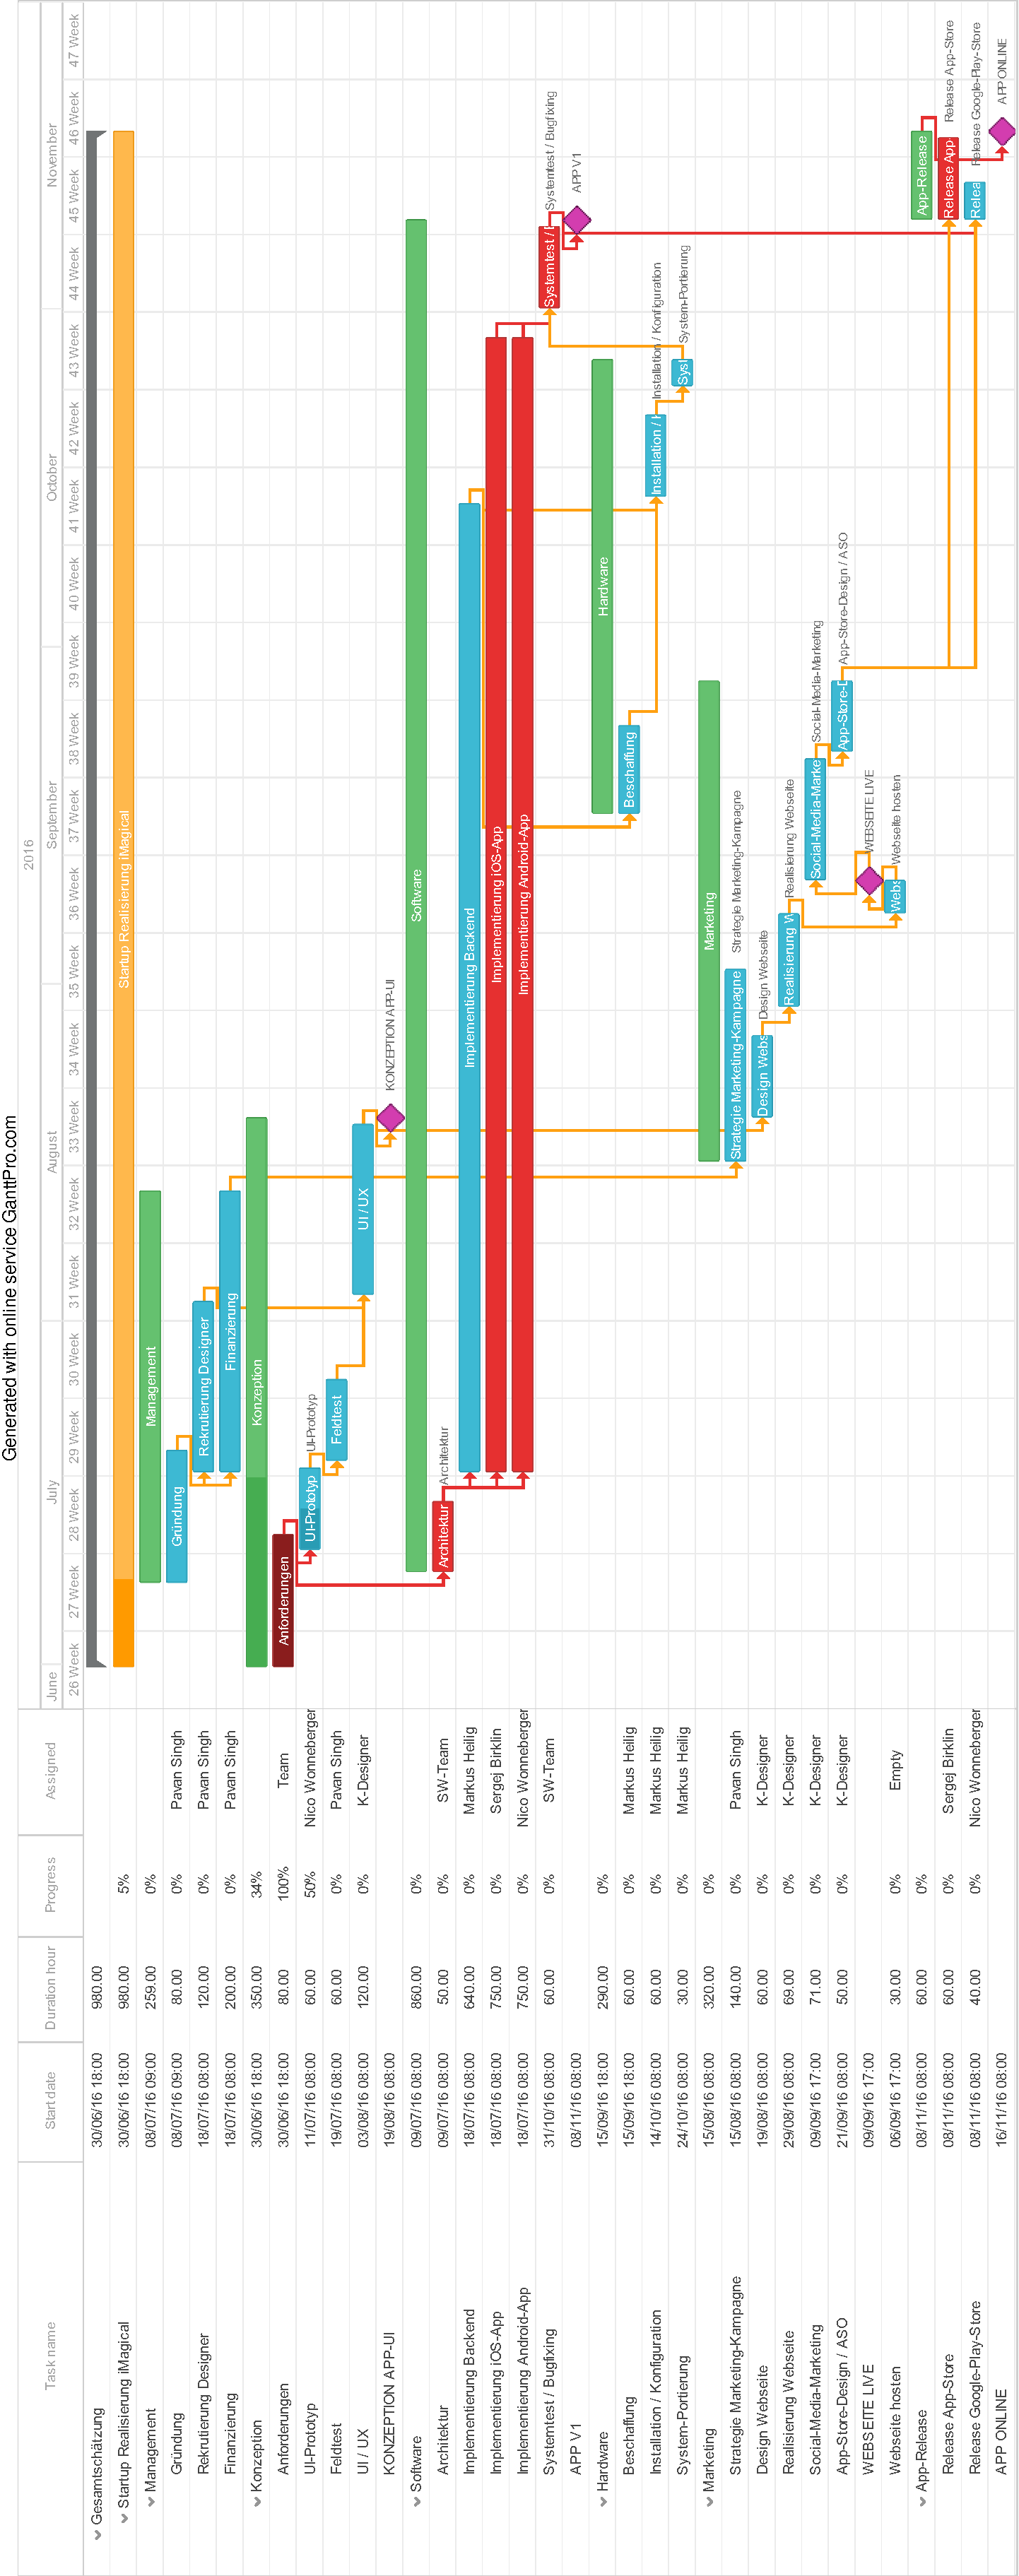
\includepdf{assets/gantt} 

\chapter{Chancen und Risiken}
Nicht wenige Menschen müssen in den ersten Jahren ihr Unternehmen wieder aufgeben. Dies liegt nicht immer an Wirtschaftskrisen, sondern ist oftmals eine Folge von schlechtem Management und Fehleinschätzungen. Dazu gehört auch, dass man die Chancen und Risiken des Unternehmens rational abwägen kann und passende Entscheidungen trifft. Eine Möglichkeit, Chancen und Risiken in Verbindung mit den eigenen Stärken und Schwächen zu quantifizieren, ist die sogenannte SWOT-Analyse. Im Folgenden soll dies an einem anschaulichen Beispiel verdeutlicht werden.

\begin{center}
	\begin{table}[htbp!]
	\centering
		\begin{tabular}{| M{2cm} | M{6cm} | M{6cm} |}
		\hline
			\textbf{ } & \textbf{Stärken} (Strength) & \textbf{Schwächen} (Weakness) \\ \hline
			\textbf{Chancen} (Opportunities)
			& \begin{itemize}
				\item []
				\item enge Kundenbindung
				\item durch kurze Entscheidungswege Flexibilität erhöhen
			\end{itemize}
			& \begin{itemize}
				\item flexibel u. unabhängig
				\item ehrgeizig u. ambitioniert
			\end{itemize}
			\\ \hline
			
			\textbf{Risiken} (Threats) 
			& \begin{itemize}
				\item relativ hohe Eintrittsbarrieren im Nieschenmarkt
				\item Erweiterung der Technologieplattform
			\end{itemize}
			& \begin{itemize}
				\item Investorensuche zur Eigenkapitalstärkung
				\item Kooperationen (fehlendes Know-How einholen)
			\end{itemize}
			\\ \hline
		\end{tabular}
		\caption{SWOT-Analyse}
		\label{table:swot}
	\end{table}
\end{center}

Die SWOT-Analyse in Tabelle \ref{table:swot} verdeutlicht zum Beispiel, dass das Gründungsteam von \textit{Imagical} sehr flexibel ist. Im Team werden kurze Kommunikationswege benutzt und muss nicht erst einige Stunden oder gar Tage auf eine Antwort warten. Vielleicht könnte  man es als Schwäche ansehen, dass das Team sehr klein und unstrukturiert wirkt. Aber auch hier sollte man die Schwäche ausnutzen und sich als junges und dynamisches Startup Team präsentieren.

Als Risiko kann natürlich gesagt werden, dass es durchaus mächtige Wettbewerber in diesem Markt gibt. Falls man sich jedoch als Nischenprodukt positionieren kann, sinkt der Wettbewerb indirekt und stellt anderen Startups im Nischenmarkt höhere Barrieren auf.
\chapter{Finanzplanung und Finanzierung}

Wie im Abschnitt „Notwendige Ressourcen“ im Kapitel „Geschäftsplanung und Organisation“ zu entnehmen ist, fallen folgende Kosten an: \\

\begin{tabular}{lc}
  \textbf{Kostenart} & \textbf{Kosten} \\
  \hline
  Macbooks & 4196{\euro} (einmalig) \\
  Gründungskosten UG & 2000{\euro} (einmalig) \\
  Arbeitsräumen im Gründerlabor unserer Hochschule & 0\euro \\
  private Grundverpflegung am Anfang & 4000\euro \\
  Reisen und Unterkunft (geschäftlich) & 300\euro \\
  Werbematerial, Flyer und Poster & 50\euro \\
  Patente & 0\euro \\
  Bargeldbestand & 500\euro \\
  Software-Lizenzen & 0\euro \\
  Weiterbildung & 0\euro \\
  Serverkosten & 100\euro \\
  Marketing & 300\euro \\
  Freelancer & 1000\euro \\
  \hline
  \textbf{Einmalkosten} & 6196{\euro} \\
  \textbf{monatliche Kosten} & 6250\euro \\
  \hline  \\
 \end{tabular}

Diese Kosten beziehen sich auf die Anfangsphase. Mit der Weiterentwicklung des Unternehmens fallen neue bzw. andere Kosten an.

Bei diesem Kostensatz lässt die durchaus pessimistische Einschätzung der monatlichen Einnahmen an knapp 17.000{\euro} zum Entschluss kommen, dass das Vorhaben sich finanziell lohnt. Vor allem das starke Potential im Einnahmenbereich - wie im Abschnitt „Erlösstruktur“ dargestellt - lässt auf diese Erkenntnis schließen.
Für den Anfang bringt jedes Teammitglied 2000{\euro} in das Vorhaben (Einlagen der Gründer), sodass die einmaligen Kosten hierfür abgedeckt werden. Für die monatlich anfallenden Kosten wird es allerdings schon schwierig. Jedoch sollte es bei diesen verhältnismäßig kleinen Summen möglich sein, Investoren gegen eine Beteiligung zu finden, die die monatlichen Kosten stemmen. Das miteingehende Mitspracherecht der Investoren wird aufgrund deren Erfahrungen durchaus begrüßt. Dieses Vorhaben verlangt angesichts der Fachkräfte im Team keine extremen finanziellen Aufwendungen. Dennoch ist es ein risikoreiches Vorhaben, für das wir keinen Kredit aufnehmen möchten, sondern das Fremdkapital ausschließlich von Investoren reinbringen lassen möchten. Aufgrund der oben geschilderten Erlös-Prognosen und der Marktanalyse kommen wir zu dem Entschluss, dass das Vorhaben wirtschaftlich als lohnenswert eingestuft werden kann und die Risiken vergleichsweise niedrig ausfallen.



\pagenumbering{Roman}
\begin{appendix}
\chapter{Screen-Designs}

\begin{center}
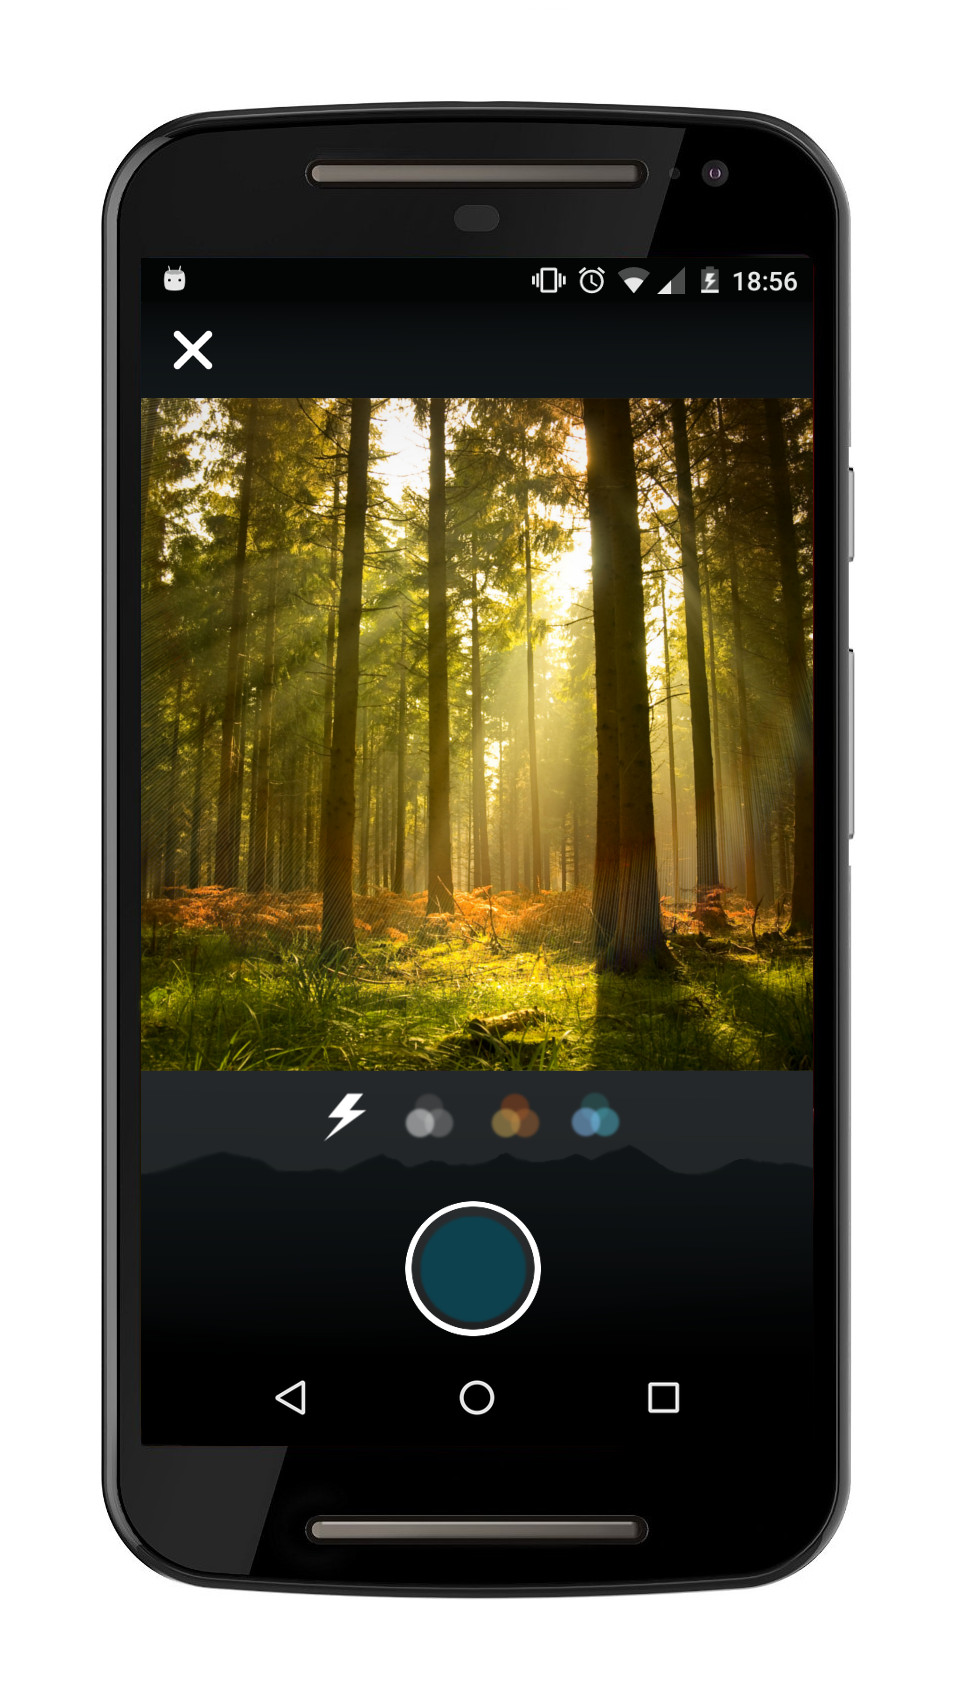
\includegraphics[width=0.37\textwidth]{assets/Screen-Camera.jpg}
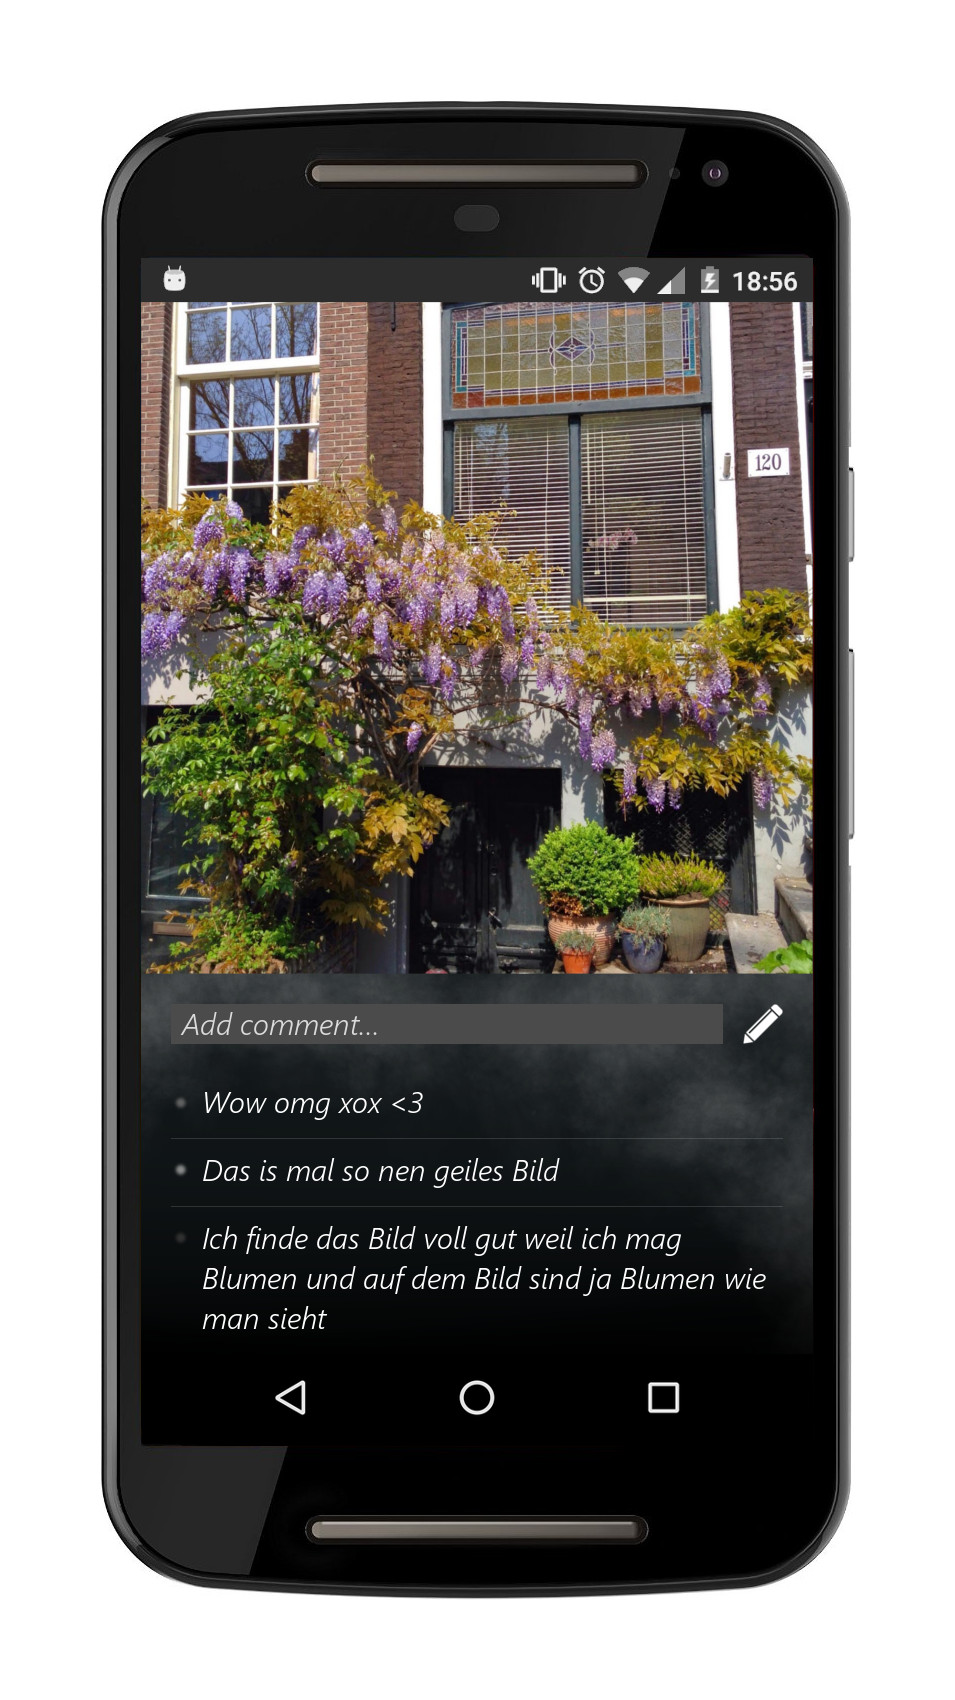
\includegraphics[width=0.37\textwidth]{assets/Screen-Image.jpg}

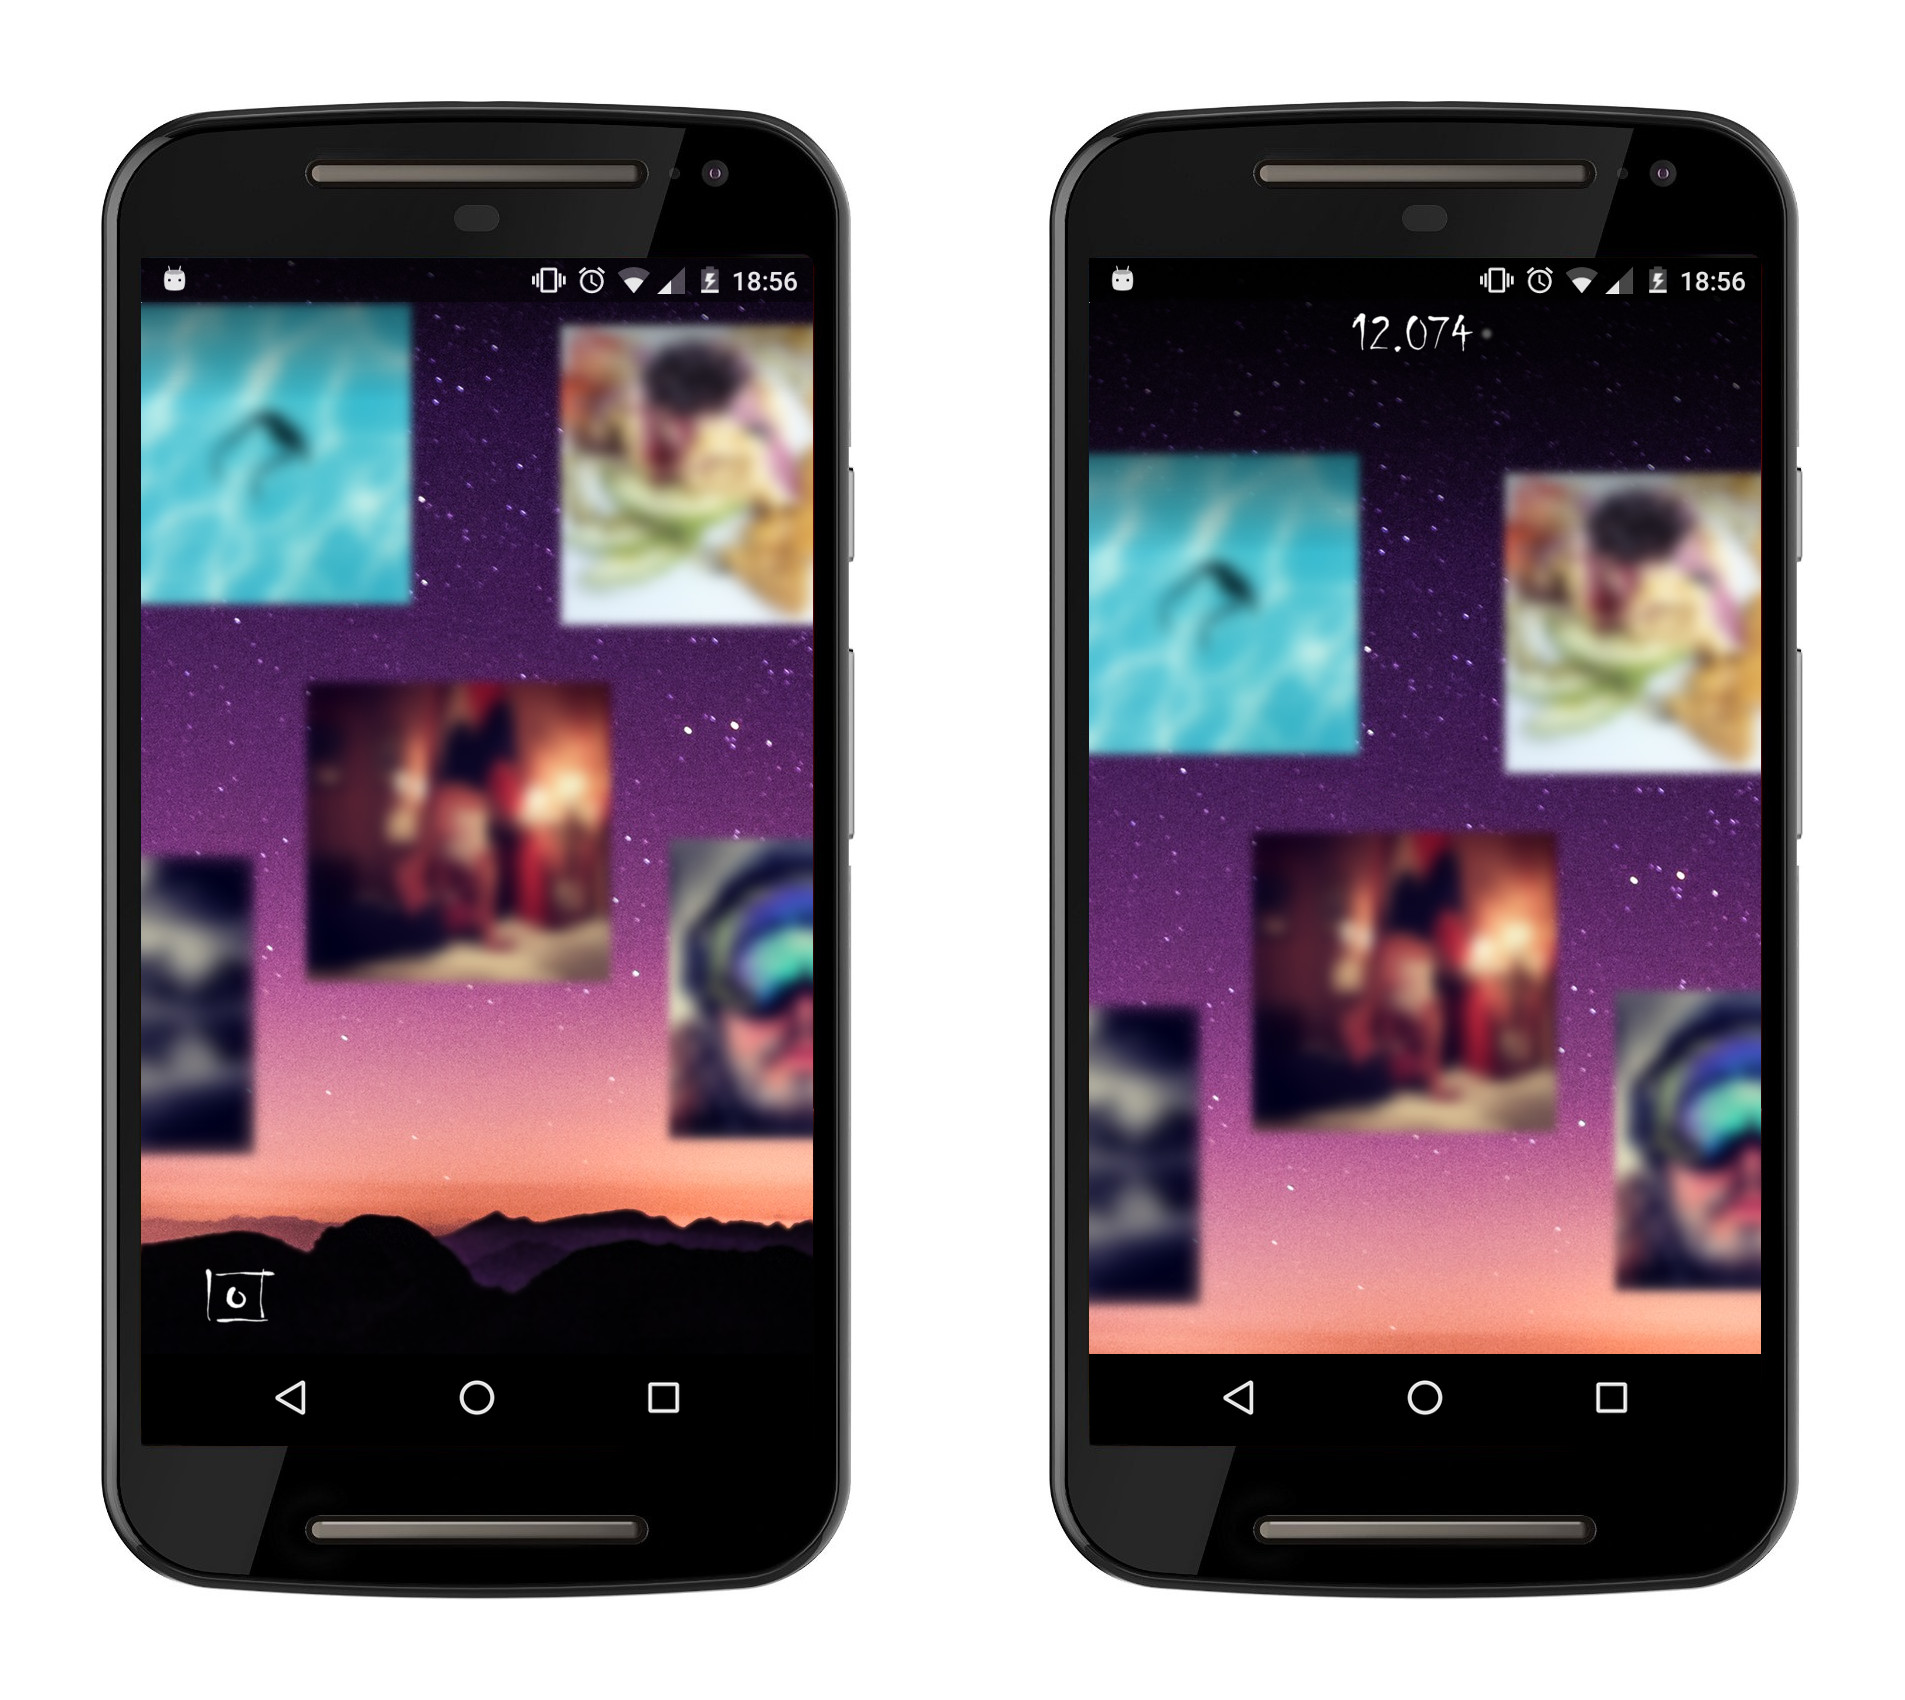
\includegraphics[width=0.74\textwidth]{assets/Screen-Home.jpg}
\end{center}


\includepdf[pages={1-13}]{assets/CreativeBrief.pdf}
\end{appendix}

\end{document}